%!TEX root = ../emo.tex
\section{Preliminary Final-Quality Assessment}
\label{sec:results}
In this section, we perform experiments to study, with regards to final quality, the main points on \nasbench discussed in the previous section. Initially, we demonstrate that with a reduced number of repetitions we are still able to satisfactorily assess relative performance of the algorithms considered here. Next, we compare the algorithms we consider from a final-quality perspective. Additionally, we examine the consequences of limiting evaluation variability. Lastly, we discuss the effects of extending the parameter space to explicitly handle a variable number of nodes.
%show how the proposed approach enriches the insights obtained by the benchmark, allowing us to compare algorithms and their search dynamics. 
%Finally, we shortly discuss the architectures selected by the different NAS algorithms.

The following experiments evaluate and compare the best-performing techniques reported in \nasbench, namely regularized evolution~(RE) and SMAC. In this study, we also include \irace, an AC that was not evaluated in the  \nasbench proposal. All NAS algorithms are run on four 24-core Intel Xeon Gold 6252 CPUs running @ 2.10GHz, with 128GB of RAM. We compare all algorithms based solely on TPU time, following the original work. 
%\leslie{We note that, as previously discussed, SMAC requires much more sequential CPU time than the remaining algorithms.}{[creo que esto no deberia ir aqui]} 
RE and SMAC are run using the code  provided by \nasbench. Additionally, both RE and SMAC are evaluated using parameter settings that showed to lead to good performance in the original \nasbench work~\cite{YinKleChrReaMurHut2019nasbench}. For fairness, we preliminarily assessed the performance of \irace in \nasbench and selected suitable hyperparameters for its application to a final-quality NAS setup. Details of the configuration process and the hyperparameters used are given in supplementary material.%
\footnote{\url{https://github.com/carlosemv/anytime-nasbench-cec2021}}

%%%
%%%
%%%
%%%
\subsection{Effect of the Number of Repetitions}

We start our assessment discussing the effect of the number of repetitions adopted for algorithm evaluation in \nasbench. We aim at reproducing as best as possible the experiments presented in the original \nasbench paper. Nevertheless, we are constrained by the computational overhead incurred by the sequential nature of SMAC and thus, we are unable to execute the 500 runs of SMAC in our computational setup. We include in the supplementary material runtime statistics for all runs performed here. In the following, we assess if the NAS techniques can be evaluated using fewer runs and if these results are comparable to the ones in the original \nasbench work.

Figure~\ref{fig:ecdf-repetitions} shows the ECDFs for final quality, measured as mean test regret, of 20~(solid) and 500~(dashed) runs of RE~(green) and \irace~(blue). 
%Both algorithms run under the setup described in the \nasbench proposal. 
%\leslie{Given the computational overhead incurred by the sequential nature of SMAC, we are unable to execute it for 500 runs in our computational setup.}{} 
Regarding RE, we remark that its performance after 500 executions~(dashed green curve) matches the report in the original \nasbench assessment. More importantly, the comparison between ECDFs produced with 20 or 500 repetitions for the algorithms highlights two important insights. First, the ECDFs for both algorithms are lowered when a larger number of repetitions is adopted. Indeed, this effect is observed progressively if we increase the number of repetitions gradually, as reported in the supplementary material. Second, the relative performance between \irace and RE is not greatly affected by the number of repetitions, with the differences in ECDFs following similar patterns. 

\begin{figure}[!t]
\centering
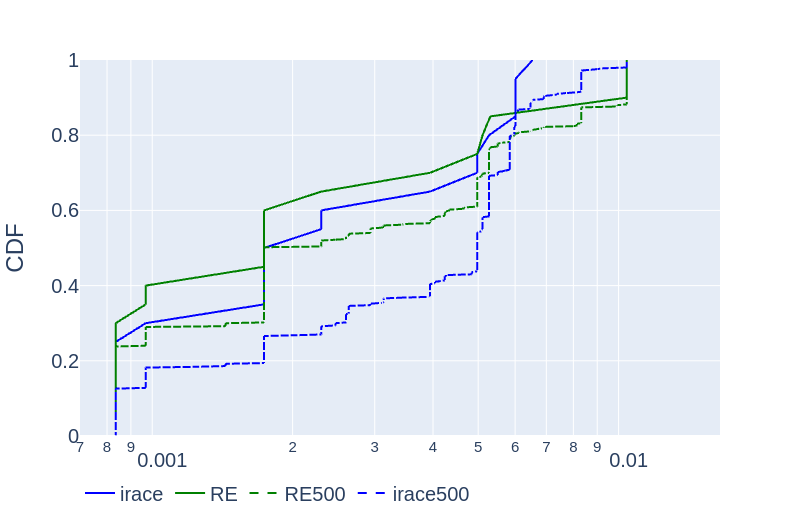
\includegraphics[width=0.8\linewidth, clip=true, trim=45px 20px 75px 50px]{imgs/ecdf-repetitions.png}
\caption{Empirical cumulative distribution function~($x$-axis) of the mean final regret~($y$-axis) assessing the effect of reducing the number of repetitions from 500~(dashed) to 20~(solid) for selected algorithms. Green: RE; blue: irace.}
\label{fig:ecdf-repetitions}
\end{figure}

\subsection{Comparing Algorithms for Final Quality}
%\leslie{}{[I think this should go in the next section, no?]} 
Figure~\ref{fig:ecdf-original} depicts the ECDFs for final quality, measured as mean test regret, of 20 runs of \irace, RE, and SMAC. Once again, all algorithms are run under the setup described in the \nasbench proposal with the exception of the number of runs, reduced for these experiments from 500 to 20.
Concerning SMAC, results differ w.r.t. the original \nasbench assessment given a change we adopt in the evaluation for comparison fairness. Specifically, the original assessment of SMAC considered a single evaluation of each configuration arguing that this led to faster convergence than multiple evaluations. We believe that this faster convergence is an effect of the limited variability provided by \nasbench and thus using such strategy may benefit all algorithms. As we will discuss in the following sections, that approach not only speeds convergence for SMAC, but leads to an improvement in its anytime performance. %Nevertheless, we remark that running SMAC with single evaluation for 20 runs produces an ECDF that follows a pattern similar to the ECDF reported in \nasbench for 500 runs.
\begin{figure}[!t]
\centering
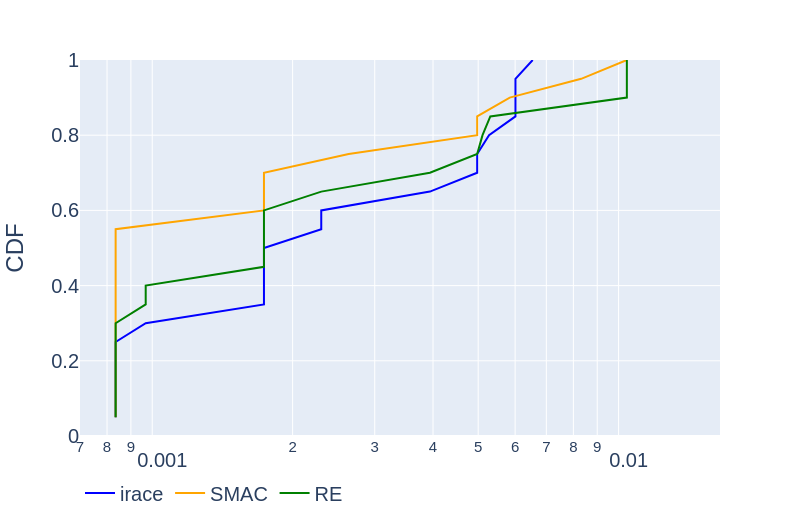
\includegraphics[width=0.8\linewidth, clip=true, trim=45px 20px 75px 50px]{imgs/ecdf-fnn-nocache.png}
\caption{Empirical cumulative distribution function~($x$-axis) of the final regret~($y$-axis) from 20 runs of each algorithm.}
\label{fig:ecdf-original}
\end{figure}

Concerning results given in Figure~\ref{fig:ecdf-original}, the comparison between \irace and the remaining algorithms shows that RE and SMAC are able to find better-performing architectures more often than \irace. However, \irace less often returns poor-performing architectures compared to RE and SMAC. Interestingly, SMAC outperforms not only \irace, but also RE, which had not been reported in the \nasbench evaluation. We believe this is due to the single versus multiple evaluation per candidate previously discussed, as follows. In~\cite{YinKleChrReaMurHut2019nasbench}, authors report that single evaluation speeds up convergence for SMAC. In search optimization, it is rather common that improving convergence speed without accounting for anytime performance leads to a decrease in final-quality performance. In addition, it is important to remark that the stopping criterion adopted does not include CPU time, hence the overhead incurred by learning in SMAC is not accounted for. 

For overall conclusions, we compare algorithms based on the area between their ECDF and the y-axis. The smaller the value, the better the performance of the algorithm.
%, indicating that every run from an algorithm achieved the minimum regret available in the benchmark. 
Table~\ref{tab:ecdf} groups results by experimental setup~(top) and algorithm~(bottom). The original setup discussed in this section is labeled~\textbf{O}~(\textit{original}). For this setup, SMAC is the best-ranked algorithm, followed by \irace and RE.
%In more detail, the AUC of the ECDF for each algorithm under each setup is given in parentheses. Results are groupby by experimental setup~(top) or algorithm~(bottom). 
We performed a Friedman non-parametric test with 98\% confidence and Nemenyi's posthoc test. When statistical significance is observed, best-ranked levels in Table~\ref{tab:ecdf} are highlighted in boldface, along with algorithms that are not statistically different to them.
Under the setup considered in this section, no statistical difference between the algorithms can be observed. 

\subsection{Evaluation Variability }
\label{sec:caching}
As previously discussed, the performance estimation required to assess the quality of an architecture requires multiple evaluations to be precise. 
%On the other hand, fewer evaluations are required when smaller variance is observed.} 
In \nasbench, the variability of the evaluations of the sampled architectures is represented only by three evaluation seeds. 
%\leslie{over only one data set}{}. \leslie{}{ 
Given this characteristic of \nasbench, we can consider storing evaluation results~(caching) to use the saved TPU time to evaluate more candidate architectures. 
This is essentially equivalent to the evaluation strategy defined in the experimental setup of SMAC in the original evaluation of \nasbench. In this section, we assess algorithms setting to one the maximum number of evaluations per architecture.
Though only SMAC has a hyperparameter to limit the number of function evaluations per configuration, we implement caching within the benchmark querying API for RE and \irace. 
%was set to one allowing only one evaluation as performance measure.

Table~\ref{tab:ecdf} shows results for the setup discussed in this section labeled as \textbf{C}~(short for \textit{caching}). 
Results grouped by experimental setup~(top) show that the relative performance of the algorithms is not altered by this factor alone. Yet, results grouped by algorithm~(bottom) demonstrate that the performance of all algorithms is much worsened when the caching strategy is adopted, though no statistical difference is observed w.r.t. other setups. We remark that \irace and RE were originally configured for the setup without caching, which could affect their performance in the caching setup. Interestingly, SMAC performs better by not using caching even having been configured for the caching setup in the original \nasbench assessment. Furthermore, it is also important to remark that \irace bases its search on statistical tests, which require variability to work. In a sense, though caching allows \irace to better explore the NAS search space, it also impairs the exploitation capability of the algorithm.
% RE, in particular, presents its worse performance among all experimental setups considered. Interestingly, if caching and variable-size encoding are adopted simultaneously, SMAC is able to achieve its best results among all experimental setups, and the performance of RE is not as poor as before. Conversely, \irace presents its worst performance. 
%Altogether, the results summarized in Table~\ref{tab:ecdf}~(bottom) evidence how different experimental design choices can have different effects on the final performance of these NAS algorithms. 

\begin{table}[!t]
    \centering
        \caption{ECDF analysis grouped by experimental setup~(top) and algorithm~(bottom). O: original; VS: variable-sized; C: caching; CVS: caching \& variable-sized. Best-ranked levels are highlighted when statistically different than the others. Values in parentheses are multiplied by $10^{4}$.}
    \label{tab:ecdf}

    \scalebox{0.825}{
    \begin{tabular}{r|r|r|r}
    \toprule
     O $\,$ & SMAC (23)$\,$ & $\,$\irace (28)$\,$  & RE (31)$\,$  \\
    \midrule
    VS $\,$ & $\,$\textbf{SMAC (18)}$\,$ & $\,$\irace (46)$\,$ & RE (47)$\,$ \\
    \midrule
    C $\,$ & $\,$ SMAC (34)$\,$ & $\,$\irace (50)$\,$ & RE (55)$\,$ \\
    \midrule
    CVS $\,$ & $\,$ \textbf{SMAC (20)}$\,$ & $\,$\irace (42)$\,$ & $\,$ RE (50)$\,$ \\
    \bottomrule
    \end{tabular}
    }
    \\[1em]
    \quad
    \scalebox{0.85}{
        \begin{tabular}{r|r|r|r|r}
        \toprule
            RE$\,$ & O (31) & VS (47) & $\,$CVS (50) & C (55)  \\
        \midrule
            \irace & O (28) & $\,$CVS (42) & VS (46) & C (50) \\
        \midrule
            SMAC$\,$ & $\,$ VS (18) & CVS (20) & O(23) & C (34)  \\
        \bottomrule
            % \multicolumn{5}{c}{}\\[0.17cm]
        \end{tabular}
}\end{table}

%%%
%%%
%%%
%%%
\subsection{Including the Number of Nodes in the Design Space}
The design space adopted in the original \nasbench considers a fixed-size encoding of
network architecture. It is important to note that, though the encoding is fixed-size, 
the final architecture they encode is variable in size. Yet, search algorithms are blind to this 
decoupling between architecture and its representation. We then include the number of
nodes as a parameter in the design space that determines the dimensions of
the adjacency matrix and node label list. Concerning final-quality ECDF analysis grouped by
experimental setup given in Table~\ref{tab:ecdf}~(top) for this setup~(labeled \textit{variable-sized}, \textbf{VS}), the relative performance of the algorithms is not affected. Yet, SMAC is now able to significantly outperform the remaining algorithms. In more detail, results grouped by algorithm~(bottom) show that SMAC greatly benefits from the variable-sized approach, whereas RE and \irace worsen their performance. 

Regarding RE and SMAC, these results are consistent with our previous discussion on the benefits of ACs. In more detail, the variable-size approach poses higher difficulty due to the larger parameter space and/or the conditional dependencies incurred by the new parameter. Under this setup, RE mutation might not be as adequate for the new design space and the algorithm is not able to define as good search trajectories as before. Conversely, ACs have been devised for scenarios that include this kind of parameter, and the performance of SMAC reflects this. Concerning \irace, we conjecture that the different probability modeling approaches adopted by SMAC (global) and \irace (local) account for the differences in performance between these algorithms for this setup. In addition, we remark that algorithms have been configured for the original setup, and hence an assessment of this encoding using reconfigured algorithms could likely alter our conclusions.

We conclude our preliminary final-quality assessment highlighting that the combination of caching and variable-sized encoding~(a setup labeled \textbf{CVS}) reveals interactions between these factors. In more detail, Table~\ref{tab:ecdf} shows that combining caching with variable-sized encoding improves over using each of these factors individually for \irace. Conversely, for RE and SMAC, caching reduces the benefits of the variable-sized encoding, even if to a much smaller extent than when we compare the original setup with using caching alone.

% \leslie{\medskip In the next section, we assess how an anytime performance perspective affects the results discussed in this final-quality preliminary assessment.}{}